\textbf{Shorten to four paragraphs.}

\begin{figure*}
\centering
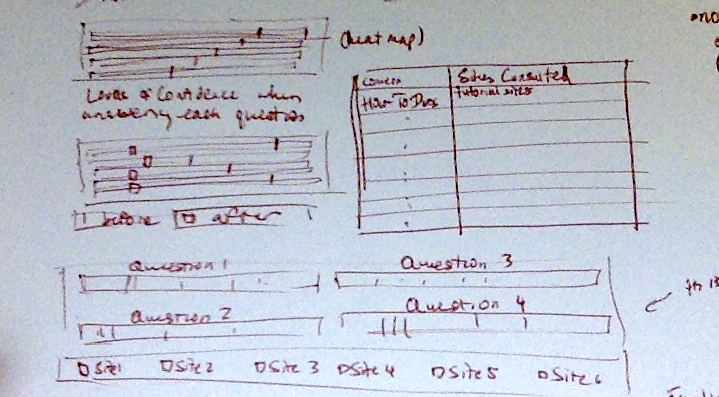
\includegraphics[width=0.7\textwidth]{figures/top_of_page}
\caption{This is the figure that goes at the top of the page}
\label{fig:top_of_page}
\end{figure*}

Include the major insights that developers had during the study.
For example:
there's a new major version;
there's an examples repository that wasn't clearly shown;
there's a Google Groups page for the project;
the docs are actually pretty usable.
From this (and hopefully other insights) we see that a surface appearance of a package takes a while to build up accurately, and might require looking at a package from multiple different angles.
We think that it need not take so much time.

Not all developers seemed to agree on what information sources were best.
Part of this is likely because of prior knowledge.
One of the participants chose to look at the IRC channels for the package.

I want to touch upon each of the following.

What questions are participants least confident answering?

What are the most authoratative sources for answering each question?

What do they approximate to aggregate?

How much do participants' perceptions of documentation change?  And how much do their opinions change?

And what does this all suggest for what's broken for information presentation, and the design of programmers' front-end to the web?
